%%%%%%%%%%%%%%%%%%%%%%%%%%%%%%%%%%%%%%%%%%%%%%%%%%%%%%%%%
% Niniejszy plik przedstawia przykładowy skład 
% pracy dyplomowej na Wydziale Matematyki PWr. 
% 
% Autorzy: 
% Damian Fafuła
% Michał Kijaczko
% Jakub Michalczak
% Maciej Miśta
% Dagmara Nowak
% Tomasz Skalski
% Wojciech Słomian
%
%% Data utworzenia: 8.05.2018
% Numer wersji: 1
%
% Poniższą formatkę można rozpowszechniać i edytować 
% pod warunkiem zachowania numeru wersji, 
% informacji o autorach i dodaniu informacji 
% o wprowadzonych zmianach.
%
%%%%%%%%%%%%%%%%%%%%%%%%%%%%%%%%%%%%%%%%%%%%%%%%%%%%%%%%%
% Domyślną opcją jest: praca magisterska, język polski.
% W przypadku pracy pisanej w języku angielskim dodajemy 
% opcję [english].
% Dla pracy licencjackiej dodajemy opcję [licencjacka].
% Dla pracy inżynierskiej dodajemy opcję [inzynierska].
% Dopuszczalne są podwójne opcje, np. [licencjacka, english].
% Opcje dodajemy w kwadratowym nawiasie przy \documentclass.
%
%
%%%%%%%%%%%%%%%%%%%%%%%%%%%%%%%%%%%%%%%%%%%%%%%%%%%%%%%%%
\documentclass[]{pwr_wmat_praca_dyplomowa}
%%%%%%%%%%%%%%%%%%%%%%%%%%%%%%%%%%%%%%%%%%%%%%%%%%%%%%%%%
%              DANE DO PRACY
%
% W przypadku pracy dyplomowej w języku angielskim nie jest konieczne 
% wypełnianie pól: \tytul{}, \kierunek{}, \specjalnosc{}, 
%                  \streszczenie{}, \slowakluczowe{}.
%%%%%%%%%%%%%%%%%%%%%%%%%%%%%%%%%%%%%%%%%%%%%%%%%%%%%%%%%
%
% Imię i nazwisko autora
\autor{Marta Janik}
%
% Tytuł pracy dyplomowej 
\tytul{Wycena opcji Amerykańskich o dyskontowaniu zależnym od cen akcji w modelu Blacka-Scholesa za pomocą metod Monte Carlo} 
\tytulang{Pricing of American option type omega clock}
%
% Tytuł / stopień / imię i nazwisko opiekuna
\opiekun{prof. dr hab. Zbigniew Palmowski}
%
% Kierunek studiów wybieramy spośród następujących:
% 1) Matematyka
% 2) Matematyka i Statystyka
% 3) Matematyka stosowana
\kierunekstudiow{Matematyka}
%
% Kierunek studiów po angielsku wybieramy spośród następujących:
% 1) Mathematics
% 2) Mathematics and Statistics
% 3) Applied Mathematics
\kierunekstudiowang{Mathematics}
%
% Specjalność wybieramy spośród następujących: 
% KIERUNEK: Matematyka
% 1) Matematyka teoretyczna,
% 2) Statystyka matematyczna,
% 3) Matematyka finansowa i ubezpieczeniowa,
%
% KIERUNEK: Matematyka i Statystyka
% 4) Matematyka,
% 5) Statystyka i analiza danych, 
%
% 6) -- (w przypadku braku specjalizacji).
\specjalnosc{Matematyka finansowa i ubezpieczeniowa} 
%
% Specjalność w języku angielskim wybieramy spośród następujących:
% KIERUNEK: Matematyka
% 1) Theoretical Mathematics,
% 2) Mathematical Statistics,
% 3) Financial and Actuarial Mathematics,
%
% KIERUNEK: Matematyka i Statystyka
% 4) Mathematics,
% 5) Statistics and Data Analysis,
%
% KIERUNEK: Applied Mathematics
% 6) Financial and Actuarial Mathematics, 
% 7) Mathematics for Industry and Commerce,
% 8) Computational Mathematics,
% 9) Modelling, Simulation and Optimization.
%
% 10) -- (w przypadku braku specjalizacji).
\specjalnoscang{Financial and Actuarial Mathematics} 
%
% Krótkie streszczenia po polsku i angielsku
% - nie dłuższe niż 530 znaków.
\streszczenie{Opcje typu omega clock zostały po raz pierwszy zaproponowane przez N. Rodosthenousa i H. Zhanga w 2017. Ten instrument różni się od dotychczas znanych derywatywów tym, że przy wycenie występuje zmienna stopa procentowa zależna od ceny instrumentu podstawowego. Celem pracy jest wyznaczenie ceny tej opcji. Do wyceny użyto metod Monte Carlo, a dokładnie algorytmu zaproponowanego przez Broadiego i Glassermana. Jest to pierwsza w historii wycena opcji typu omega clock.}
\streszczenieang{Option type Omega clock were first proposed by N. Rodosthenous and H. Zhang in 2017. This instrument differ from others derivatives with discounting during pricing, the interest rate depend from price of option. The main goal of this thesis is finding the price of this option. To pricing was used Monte Carlo method, exactly Broadie Glasserman's algorithm. It is the first valuation of option type Omega clock in history.}
%
% Podajemy najważniejsze słowa kluczowe po polsku i angielsku
% - w obu przypadkach, nie więcej niż 150 znaków.
\slowakluczowe{Opcje amerykańskie typu omega clock, Model Blacka-Scholesa, Metoda Broadie Glassermana}  
\slowakluczoweang{American option type omega clock, Black-Scholes model, Broadie Glasserman method}
%
%
%%%%%%%%%%%%%%%%%%%%%%%%%%%%%%%%%%%%%%%%%%%%%%%%%%%%%%%%%
% Definicje, lematy, twierdzenia, przykłady i wnioski
% Komendy wywołujące twierdzenia, definicje, itd., 
% czyli 'theorem', 'definition', 'corollary', itd., 
% można zmienić wedle uznania.
\theoremstyle{plain}
\newtheorem{theorem}{Twierdzenie}
\numberwithin{theorem}{chapter}
\newtheorem{lemma}[theorem]{Lemat} 
\newtheorem{corollary}[theorem]{Wniosek}
\newtheorem{fact}[theorem]{Fakt}
\theoremstyle{definition}
\numberwithin{theorem}{chapter}
\newtheorem{definition}[theorem]{Definicja} 
\newtheorem{example}[theorem]{Przykład}
\newtheorem{note}[theorem]{Uwaga}
%%%%%%%%%%%%%%%%%%%%%%%%%%%%%%%%%%%%%%%%%%%%%%%%%%%%%%%%%

\usepackage{tikz}
\newcommand\encircle[1]{%
  \tikz[baseline=(X.base)] 
    \node (X) [draw, shape=circle, inner sep=1] {\Large{\strut #1}};}
    
\newcommand\mkcircle[1]{%
  \tikz[baseline=(X.base)] 
    \node (X) [draw, shape=circle, inner sep=0] {\large{\strut #1}};}
    
\newcommand\enrectangle[1]{%
    \tikz[baseline=(X.base)]
       \node (X) [draw, shape=rectangle, inner sep=1]{\strut #1};}

%%%%%%%%%%%%%%%%%%%%%%%%%%%%%%%%%%%%%%%%%%%%%%%%%%%%%%%%%
%%%%%%%%%%%%%%%%%%%%%%%%%%%%%%%%%%%%%%%%%%%%%%%%%%%%%%%%%
\begin{document}
\frontmatter
\maketitle
\mainmatter
\tableofcontents
\listoffigures
\listoftables

{\backmatter \chapter{Wstęp}}

Opcje nie są nowym instrumentem finansowym. Ich historia sięga czasów starożytnej Grecji - pierwsze informacje dotyczące opcji można znaleźć w $I$ księdzie \textit{Polityki} Arystotelesa, który opisał historię znanego matematyka Talesa z Miletu. Przewidział on obfite zbiory oliwek w następującym roku. Spodziewając się związanego z tym dużego popytu na wykorzystywanie pras do oliwek, przed sezonem zbiorów wykupił prawo ich używania. Spekulacja okazała się słuszna - zbiory były obfite, co umożliwiło Talesowi odnajmowanie pras po wyższej cenie\footnote{Arystoteles,\textit{Polityka}, Warszawa 1964}. Pierwszy stosunkowo dobrze rozwinięty rynek instrumentów pochodnych powstał w XVII w. w Holandii. Pomimo tak długiej historii rynków opcyjnych praw nimi rządzących zaczęto szukać dopiero w XIX wieku. Przełomowym wydarzeniem było wprowadzenie modelu do wyceny europejskiej opcji standardowej na akcje spółek niewypłacających dywidendy wyprowadzonego przez Fishera Blacka i Myrona Scholesa w 1973 roku. Od tego czasu powstało wiele rozszerzeń i modyfikacji tego modelu do wyceny derywatywów innych niż standardowe.

Rynek opcji wciąż intensywnie się rozwija, o czym świadczy wprowadzanie nowych instrumentów pochodnych. Jednym z takich przykładów są opcje typu omega clock. Zostały one po raz pierwszy zaproponowane przez N. Rodosthenousa i H. Zhanga w 2017. Ten instrument różni się od dotychczas znanych derywatywów tym, że przy wycenie występuje zmienna stopa procentowa zależna od ceny instrumentu podstawowego.

Do ustalania ceny niektórych opcji istnieją powszechnie znane narzędzia analityczne, jednak wiele z nich ma skomplikowaną funkcję wypłaty i jest wycenianych za pomocą metod numerycznych. W tej pracy do wyceny opcji typu omega clock użyto metod Monte Carlo, a dokładnie algorytmu opartego na metodzie zaproponowanej przez Broadiego-Glassermana w 1997 roku. Ta metoda estymuje premię opcji używając drzewa cenowego, które wyznacza i powiela możliwe trajektorie ceny instrumentu podstawowego. W wyniku otrzymuje się górne i dolne estymatory, które zbiegają do prawdziwych cen opcji.

Celem pracy jest wyznaczenie po raz pierwszy w historii ceny amerykańskiej opcji typu omega clock na akcje. W pracy znajdują się teoretyczne wzory na estymatory premii opcji i estymowanej ceny, a także wyniki przeprowadzonych symulacji dla danych rzeczywistych.

Przy pisaniu pracy korzystano z literatury źródłowej dotyczącej opcji i ich wyceny. Szczególnie zostały wykorzystane książki: Paula Glassermana \textit{,,Monte Carlo Methods in Financial Engineering''}, Johna Hulla \textit{,,Kontrakty terminowe i opcje. Wprowadzenie''}, Aleksandra Werona i Rafała Werona \textit{,,Inżynieria finansowa''}, a także artykuł Marka Broadiego i Paula Glassermana \textit{,,Pricing American-style securities using simulation''}.

Praca składa się ze wstępu i czterech rozdziałów. W pierwszym przedstawiono wszystkie podstawowe informacje potrzebne do zrozumienia pracy. Zawiera on informacje o opcjach, ich podstawowy podział i funkcje wypłaty dla opcji standardowych. Następnie opisano ruch Browna, który został wykorzystany do prognozy cen akcji. W tym rozdziale opisano również model Blacka-Scholesa, który został wykorzystany do wyceny, a także metody Monte Carlo, których użyto do analizy numerycznej. W drugim rozdziale opisano opcje typu omega clock, które są wyceniane w tej pracy. Przedstawiono model, według którego będzie wyceniana. Rozdział trzeci zawiera pełny opis metody Broadiego-Glassermana oraz jej zastosowanie dla przykładowego drzewa cenowego. Rozdział czwarty, za razem ostatni i najważniejszy, przedstawia analizę numeryczną. Najpierw porównano ceny waniliowej opcji amerykańskiej wyznaczonej za pomocą zaimplementowanego algorytmu i za pomocą sprawdzonych metod, by sprawdzić poprawność metody. Następnie pokazano wycenę amerykańskiej opcji sprzedaży typu omega clock dla danych rzeczywistych.

Wszystkie analizy numeryczne mają na celu uzasadnienie poprawności zaimplementowanego algorytmu do wyceny opartego na metodzie Broadiego Glassermana i doprowadzenie do wyznaczenia sprawiedliwej premii opcji amerykańskiej sprzedaży typu omega clock.

\chapter{Wiadomości wstępne}
W tym rozdziale znajdują się informacje potrzebne do zrozumienia pracy dotyczące teorii opcji, ich wyceny i metod numerycznych.\\
Najpierw zostały opisane opcje, następnie sposób wyznaczania przyszłej ceny instrumentu podstawowego, model wykorzystywany do wyceny derywatywów oraz podstawowe informacje dotyczące metod numerycznych użytecznych do wyceny, a dokładnie metod Monte Carlo.

\section{Opcje}
%Historia?
Opcja to instrument finansowy, który można zdefiniować jako umowę pomiędzy sprzedawcą a nabywcą, która daje nabywcy prawo do kupna lub sprzedaży (w zależności od rodzaju instrumentu finansowego) określonej ilości pewnego dobra bazowego w ustalonym terminie po wyznaczonej cenie. Innymi słowy, opcja to umowa z ustalonymi warunkami, która daje nabywcy pewną możliwość.
%Ważnymi terminami dotyczącymi kontraktów opcyjnych są \textit{termin wygaśnięcia}, po którym opcja traci ważność, \textit{termin wykonania}, w który nabywca może wykorzystać swoje prawo (wykonać opcję) oraz \textit{termin rozliczenia}, który występuje zwykle dwa dni robocze po wykonaniu opcji, i do którego musi zostać przeprowadzona fizyczna wymiana dobra bazowego bądź gotówki.\\
Najstarsze kontrakty opcyjne opiewały na akcje. Obecnie instrumentami podstawowymi opcji w obrocie giełdowym są zazwyczaj: waluty obce, indeksy giełdowe czy kontrakty \textit{futures}. Na rynkach pozagiełdowych opcje są zazwyczaj dostosowywane do indywidualnych potrzeb klientów, zatem dobro podstawowe jest praktycznie dowolne.\\

Opcje można podzielić na wiele sposobów, biorąc pod uwagę różne kryteria. Pierwsze i najważniejsze rozróżnienie to podział na opcje:
\begin{itemize}
\item kupna - \textit{call}, która daje jej posiadaczowi prawo do kupna instrumentu bazowego,
\item sprzedaży - \textit{put}, która daje posiadaczowi prawo do sprzedaży tego dobra.
\end{itemize}

\noindent Drugi podział występuje ze względu na rozróżnienie terminu wygaśnięcia i wykonania opcji. Taki podstawowy podział to opcje:
\begin{itemize}
\item europejskie, które można wykonać jedynie w terminie wygaśnięcia,
\item amerykańskie, które mogą być wykonane przez cały okres ważności finansowego instrumentu pochodnego, tj. w każdym momencie od nabycia do czasu wygaśnięcia opcji.
\end{itemize}
Nazwy te mają pochodzenie historyczne i w żaden sposób nie są związane z miejscem obrotu. Warto zauważyć również, że na rynku światowym większy obrót mają opcje amerykańskie, co wynika z faktu, że opcje europejskie są podatne na manipulacje w czasie bliskim terminowi wygaśnięcia. Te dwie opcje to opcje standardowe, w żargonie finansowym nazywane również opcjami waniliowymi. Nazwa ta pochodzi od lodów waniliowych, które są \textit{najprostszym} smakiem lodów, czyli bez żadnych dodatków. Inne opcje nazywane są opcjami egzotycznymi (np. opcja azjatycka).

\paragraph{Premia opcji} Aby stać się posiadaczem opcji należy za nią zapłacić. Taka cena jest nazywana \textit{premią opcji}. Na jej wysokość ma wpływ wiele czynników, jednak najważniejszym jest funkcja wypłaty. Ta funkcja określa wysokość wypłaty jaką otrzyma nabywca w momencie jej wykonania. Funkcje wypłaty opcji podstawowych przedstawia poniższa tabela, w której $T$ - termin wygaśnięcia, $S_t$ - cena dobra bazowego w chwili $t$ ($0 \leq t \leq T$), $K$ - cena wykonania opcji (zawarta w kontrakcie).

\begin{table}[ht]
\caption{Funkcje wypłaty opcji waniliowych}
\centering
\begin{tabular}{|c|c|c|}
\hline                       
\textbf{Opcja} & \textbf{Kupna} & \textbf{Sprzedaży}\\
\hline 
\textbf{europejska} & $f_T^C = \max(S_T-K,0)$ & $f_T^P = \max(K-S_T,0)$  \\[1ex]
\textbf{amerykańska} & $f_t^C = \max(S_t-K,0)$ & $f_t^P = \max(K-S_t,0)$  \\[1ex]  
\hline 
\end{tabular}
%\caption*{\textit{Źródło: Weron&Weron}}
\label{tab:wyplata} 
\end{table}
\noindent Funkcja wypłaty związana jest z wartością wewnętrzną opcji. Natomiast na wartość zewnętrzną opcji, nazywanej inaczej czasową, mają wpływ trzy podstawowe czynniki:
\begin{itemize}
\item czas pozostający do wygaśnięcia opcji,
\item wolna od ryzyka stopa procentowa $r$,
\item zmienność ceny akcji $\sigma$, czyli miara niepewności co do przyszłych zmian cen instrumentu podstawowego.
\end{itemize}
Premia opcji to suma jej wartości wewnętrznej i zewnętrznej.

%%%%%%%%%%%%%%%%%%%%%%%%%%%%%%%%%%%%%%%%%%%%%%%%%%%%%%%%%%%%%%%%%%%%%%%%%%%55
\section{Ruch Browna}

Do wyznaczenia funkcji wypłaty, a co za tym idzie również premii opcji, potrzebna jest znajomość ceny instrumentu podstawowego $S_t$ ($t \in [0,T]$). Do tego wykorzystywany jest geometryczny ruch Browna.

\subsection{Historia}

W 1900 roku Louis Bachelier, przez wielu uważany za ojca matematyki finansów, jako pierwszy użył matematyki do przewidywania zmian ceny na rynku. W swojej pracy doktorskiej \textit{Theorie de la speculation} skupił się na prawdopodobieństwie fluktuacji cen instrumentów finansowych na giełdzie paryskiej. Do jego opisu wykorzystał ruch Browna, który został tak nazwany od nazwiska botanika Roberta Browna, który w 1827 roku zaobserwował ruch cząsteczek i go opisał. Bachelier użył tego ruchu ponieważ uznał, że zmiany ceny dobra bazowego są równie chaotyczne i nieprzewidywalne, co ruchy cząsteczek pyłku. Podstawowe własności ruchu Browna zostały udowodnione w 1905 roku przez Alberta Einsteina i równolegle w 1906 przez Mariana Smoluchowskiego, dzięki czemu ruch ten wszedł na stałe do użytku w fizyce. Dopiero Norbert Wiener (w 1927) i Paul Levy (w 1939) doprowadzili do wprowadzenia ruchu Browna do matematyki. Proces Wienera (matematyczna nazwa ruchu Browna) stał się jednym z najważniejszych modeli losowych. W ekonomii znalazł on zastosowanie do konstrukcji modeli cen giełdowych.\\

\subsection{Definicja}
Aby przedstawić formalną definicję procesu Wienera trzeba wprowadzić pewne pojęcia i założenia. \\

Przestrzeń, na której przeprowadzane są rozważania probabilistyczne, oznacza trójka probabilistyczna $(\Omega, \mathcal{F}, \mathbb{P})$, gdzie $\Omega$ to zbiór wszystkich możliwych wyników, $\mathcal{F}$ to $\sigma$-ciało podzbiorów $\Omega$, $\mathbb{P}$ to miara prawdopodobieństwa na $\mathcal{F}$. Wprowadzono również oznaczenia na przedział życia opcji, a dokładniej $\mathbb{T} = [0,T]$, gdzie $T$ - moment wygaśnięcia opcji.\\
\newline
Formalnie proces Wienera to rodzina zmiennych losowych $(W_t)_{t\in \mathbb{T}}$  określonych na jednej przestrzeni probabilistycznej $(\Omega, \mathcal{F}, \mathbb{P})$ jest to zatem pewien proces stochastyczny. Dla pewnych ustalonych $\omega \in \Omega$ funkcja $t \rightarrow W_t(\omega)$ jest trajektorią procesu. Definicja procesu Wienera to:

\begin{definition}[proces Wienera]\footnote{J.Jakubowski, A.Palczewski, M.Rutkowski, Ł. Stettner, \textit{Matematyka finansowa. Instrumenty pochodne}, Warszawa 2018}
Standardowym procesem Wienera lub krótko procesem Wienera nazywamy proces stochastyczny $W$ z czasem ciagłym, spełniający następujace warunki:
\begin{enumerate}
\item $W_0 = 0$;
\item Przyrosty procesu $W$ są niezależne, czyli dla dowolnego $n$ i dowolnego ciągu $0<t_1<\ldots<t_n$ zmienne losowe
$$ W_{t_1}, W_{t_2}-W_{t_1},\ldots, W_{t_n} - W_{t_{n-1}}$$
są niezależne;
\item Dla dowolnych $0\leq s < t$ przyrost $W_t-W_s$ ma rozkład gaussowski, a dokładniej
$$ W_t - W_s \sim N(0,t-s);$$
\item Proces $W$ jest ciągły, tzn. prawie wszystkie trajektorie procesu $W$ są funkcjami ciągłymi.
\end{enumerate}
\end{definition}

\subsection{Geometryczny ruch Browna}
Niezależność przyrostów proccesu Wienera, ciągłość jego trajektorii i inne jego własności, a także jego nieprzewidywalność (jak zauważył Bachelier) skłaniają do wykorzystania tego procesu do poszukiwania prawdopodobnej przyszłej ceny dobra podstawowego, jednak standardowy proces Wienera okazuje się mało użyteczny w finansach, dlatego w inżynierii finansowej wykorzystuje się jego różne modyfikacje. Najbardziej popularne można przedstawić za pomocą poniższego stochastycznego równania różniczkowego
\begin{equation}
\label{eq:proces}
dX_t = \mu(X_t,t)dt + \sigma(X_t,t)dW_t,
\end{equation}
gdzie $\mu$ - to współczynnik dryfu (przesunięcia), $\sigma$ - współczynnik zmienności (dyfuzji), a $X_t$ - nowy proces stochastyczny.\\

Louis Bachelier do oszacowania prawdopodobieństwa fluktuacji cen na giełdzie paryskiej wykorzystał arytmetyczny ruch Browna, czyli we wzorze (\ref{eq:proces}) przyjął zerowe oprocentowanie $\mu \equiv 0$ i stałą zmienność $\sigma$. Wówczas wzór na cenę przyjmuję postać $$ S_t = S_0 + \sigma W_t,$$ jednak bazuje on na nierealistycznym założeniu, że stopa procentowa jest zerowa oraz dopuszcza ujemne ceny. W latach 1955-59 Paul Samuelson i M.F.M. Osborne niezależnie od siebie poprawili pomysł Bachelier, przyjmując w równaniu (\ref{eq:proces}) $\mu(X_t,t)=\mu X_t$ i $\sigma(X_t,t)=\sigma X_t$. Stochastyczne równanie różniczkowe na cenę dobra bazowego przyjmuje wówczas postać
\begin{equation}
\label{eq:dSt}
dS_t = t S_t dt + \sigma S_t dW_t
\end{equation}
a taki proces $S_t$ nazwano geometrycznym (inaczej eksponencjalnym) ruchem Browna.

\paragraph{Własności} Tak zmodyfikowany proces Wienera ma wiele własności, które pozwalają dobrze kształtować ceny, a dokładnie, jeśli przyjmiemy, że $X_t$ jest eksponencjalnym ruchem Browna, wówczas:
\begin{itemize}
\item Jeśli $X_0 > 0$, to proces $X_t$ pozostaje dodatni;
\item Na poziomie zero proces $X_t$ ma barierę absorbującą, czyli jeśli w pewnym momencie $t$ osiągnie zero, to już taki pozostanie;
\item Proces $X_t$ ma rozkład lognormalny, tzn. $\ln X_t$ ma rozkład normalny z odpowiednimi parametrami średniej i wariancji (łatwo to pokazać wykorzystując postać geometrycznego ruchu Browna, postulat procesu Wienera o gaussowskich przyrostach i własności procesu normalnego).
\end{itemize}

\subsection{Proces ceny akcji}

Rozwiązując stochastyczne równanie różniczkowe (\ref{eq:dSt}) można łatwo wyznaczyć postać ceny $S_t$:
\begin{equation}
\label{eq:St}
S_t = S_0 \exp((\mu - \frac{1}{2}\sigma^2)t + \sigma W_t).
\end{equation}
Łatwo pokazać, że 
\begin{equation}
\label{eq:rozklad}
\ln S_t \sim N(\ln S_0 + (\mu-\frac{1}{2}\sigma^2)t, \sigma^2 t).
\end{equation}

\noindent Do późniejszej wyceny będziemy używać wzoru (\ref{eq:St}).

%%%%%%%%%%%%%%%%%%%%%%%%
\section{Model Blacka-Scholesa}
Wycena opcji sprowadza się do wyznaczenia jej premii. W poprzednim podrozdziale pokazano, że proces ceny $S_t$ można opisać geometrycznym ruchem Browna, skąd łatwo można wyznaczyć już funkcje wypłaty $f_t$ dla opcji standardowych. Jednak wyznaczenie sprawiedliwej premii nie może składać się z jednej obserwacji, gdyż nie byłoby to miarodajne. Pierwszym i do tej pory najbardziej podstawowym modelem wyceny jest model Blacka-Scholesa. W pracy będzie wyceniana amerykańska opcja sprzedaży akcji, dla której model w chwili $t$ przyjmuje postać
\begin{equation}
\label{eq:B-S}
\pi_t(X) = \sup_{\tau \in \mathcal{T}} \Lambda_{\tau}\{\mathbb{E}^{\mathbb{Q}}[\Lambda_{T}^{-1}\max(K-S_{\tau},0)|\mathcal{F}_{\tau}]\},
\end{equation}
gdzie $\pi_t(X)$ - premia opcji $X$ w chwili t, $\tau$ - moment stopu, $\mathcal{T}$ - rodzina wszystkich możliwych momentów stopu, $\Lambda_t$ - czynnik dyskontujący w chwili $t$, $\mathbb{Q}$ - miara martyngałowa, $\mathcal{F}_t$ - filtracja. Wszystkie potrzebne definicje zostaną przedstawione później.

\subsection{Historia}
Podstawą rynku opcyjnego jest wyznaczanie sprawiedliwych cen opcji, dlatego ciekawy jest fakt, że choć pierwszy rynek instrumentów pochodnych powstał w Holandii w XVII wieku, to praw nim rządzącym zaczęto szukać dopiero dwa wieki później. Jednak dopiero w 1973 roku nastąpił przełom, gdy Fisher Black i Myron Scholes przedstawili model wyceny waniliowych opcji europejskich na akcje spółek niewypłacających dywidendy. Było to ważne odkrycie, ponieważ do tego roku nikt nie potrafił wyznaczyć sprawiedliwej ceny opcji, co miało duży wpływ na małą płynność rynku i zmienność cen. Model Blacka-Scholesa jest pierwszym matematycznie wyprowadzonym modelem wyceny opcji na akcje.

Idea modelu Blacka-Scholesa opiera się o pozbawiony ryzyka portfel, składający się z pozycji w opcji i pozycji w akcji bazowej dla tej opcji.\footnote{J. Hull, \textit{Kontrakty terminowe i opcje. Wprowadzenie}, Warszawa 1997}

\subsection{Założenia}

W pracy będę przeprowadzać wycenę zgodnie z modelem Blacka-Scholesa, jednak żeby to było możliwe trzeba najpierw przyjąć pewne założenia: 

\begin{enumerate}
\item Brak możliwości arbitrażu (nie ma możliwości zarobienia bez ponoszenia ryzyka);
\item Wolna od ryzyka, krótkoterminowa stopa procentowa jest stała w czasie życia opcji;
\item Nie uwzględnia się kosztów transakcji ani podatków;
\item Istnieje możliwość zakupu każdej, nawet ułamkowej, ilości akcji;
\item Akcje nie wypłacają dywidendy;
\item Brak kary za zajmowanie krótkiej pozycji (np. opcja sprzedaży na akcje, których się nie ma)).
\end{enumerate}
W modelu Blacka-Scholesa przyjmujemy, że cenę dobra bazowego $S_t$ w dowolnej chwili $t$ opisuje geometryczny ruch Browna ze stałą zmiennością $\sigma$ i  stałym dryfem $\mu$ opisany za pomocą stochastycznego równania różniczkowego (\ref{eq:dSt}). Ma ona rozkład lognormalny przedstawiony wzorem (\ref{eq:rozklad}).

\subsection{Definicje}
W tej pracy będzie wyceniana opcja amerykańska, czyli taka, którą posiadacz może wykorzystać w całym czasie życia opcji. Z tego powodu potrzebujemy zaznajomić się z pojęciem momentów stopu.

\begin{definition}[Filtracja]
Filtracją nazywamy niemalejącą rodzinę $\sigma$-ciał
$$\mathbb{F} = (\mathcal{F}_t)_{t \in \mathbb{T}},$$
tzn. $\mathcal{F}_s \subseteq \mathcal{F}_t \subseteq \mathcal{F}$ dla $s<t$ i $s,t \in \mathbb{T}$
\end{definition}

\begin{definition}[Naturalna filtracja] 
Niech $(X_t)_{t \in \mathbb{T}}$ będzie procesem stochastycznym. Wówczas naturalna filtracja $\mathbb{F}^X$ to $$\mathcal{F}_t^X = \sigma(X_s: s \leq t).$$
\end{definition}

\noindent Od tego momentu przyjmujemy również, że filtracja będzie spełniała zwykłe warunki, tzn. jest prawostronnie ciągła, a dokładniej dla każdego $t$ zachodzi równość $\mathcal{F}_t = \mathcal{F}_{t_+}$, gdzie $\mathcal{F}_{t_+} = \bigcap_{t<s} \mathcal{F}_s$, oraz jest zupełna, tzn. każde $\sigma$-ciało $\mathcal{F}_t$ jest zupełne.
\newline
\newline
Zdefiniujmy teraz moment stopu.

\begin{definition}[Moment stopu]
Zmienna losowa $\tau$, $\mathcal{F}$-mierzalna, $\tau: \Omega \rightarrow \mathbb{T} \cup \{\infty\}$ jest momentem stopu względem filtracji $(\mathcal{F}_t)_{t \in \mathbb{T}}$, gdy $\forall_{t \in \mathbb{T}}$
$$ \{ \tau \leq t \} \in \mathcal{F}_t.$$ Rodzinę momentów stopu będziemy oznaczać przez $\mathcal{T}.$
\end{definition}

\noindent W pracy używamy modelu Blacka-Scholesa, który przyjmuje postać pewnej warunkowej wartości oczekiwanej względem miary martyngałowej. Aby zrozumieć definicję takiej miary, zdefiniujmy najpierw martyngał - jedną z najważniejszych klas procesów stochastycznych.

\begin{definition}[Martyngał]
Rodzina $(X_t,\mathcal{F}_t)_{t\in \mathbb{T}}$ jest martyngałem, jeśli dla $ s \leq t$, $s,t \in \mathbb{T}$ $$ \mathbb{E}(X_t|F_s) = X_s.$$
Mówiąc o $\mathbb{P}$-martyngałach sprawdzamy wartość oczekiwaną względem miary $\mathbb{P}$.
\end{definition}

\begin{definition}[Miara martyngałowa]
Miara $\mathbb{Q}$, względem której $\mathbb{E}^{\mathbb{Q}}(X_t|\mathcal{F}_s)$ jest martyngałem, jest miarą martyngałową względem procesu $X_t$.\\
Taką miarę w literaturze nazywa się prawdopodobieństwem neutralizującym ryzyko.
\end{definition}
 
We wzorze (\ref{eq:B-S}) występuje również czynnik dyskontujący w chwili $t$ oznaczony przez $\Lambda_t$. Służy on do znajdowania bieżącej wartości ceny dobra mając daną jego przyszłą wartość. Zazwyczaj dany on jest przez $\Lambda_t = e^{-\int_0^tr(t)dt}$, gdzie $r(t)$ jest daną funkcją oprocentowania.\\

\noindent W tym momencie znamy już wszystkie potrzebne definicje do wzoru na model Blacka-Scholesa przedstawionego we wstępie do tego rozdziału (wzór~(\ref{eq:B-S})).
 
%\subsection{Wyprowadzenie modelu}
%\textsc{\textcolor{red}{Pisać coś jeszcze? (O B-S)}}
 
\section{Metody Monte Carlo}

W pracy będziemy używać metod numerycznych. W modelu Blacka-Scholesa do wyliczenia ceny opcji trzeba znaleźć wartość oczekiwaną zdyskontowanych wypłat (funkcji wypłaty) względem pewnej miary martyngałowej, a do tego posłużą metody Monte Carlo.\\

Metody Monte Carlo są metodami obliczania wielkości dających się przedstawić w postaci wartości oczekiwanych pewnych rozkładów probabilistycznych.\footnote{A.Weron, R.Weron, \textit{Inżynieria finansowa. i coś dalej}} Bazują one na Mocnym Prawie Wielkich Liczb:

\begin{theorem}[Mocne Prawo Wielkich Liczb]
\label{th:MPWL}
Niech $X_1,\ldots,X_n$ będą niezależnymi zmiennymi losowymi o tym samym rozkładzie i skończonej wartości oczekiwanej (tzn. $\mathbb{E}(X_i)<\infty$, dla $i=1,\ldots,n$). Wtedy
\begin{equation*}
 \mathbb{P}(\lim_{n\rightarrow \infty}\frac{1}{n}\sum_{i=1}^n x_i = \mathbb{E}(X)) = 1.
\end{equation*}
\end{theorem}
\noindent Zatem korzystając z twierdzenia (\ref{th:MPWL}) łatwo wywnioskować, że za oszacowanie wartości oczekiwanej $X$ można przyjąć średnią empiryczną z pewną, odpowiednio dobraną liczbą obserwacji $n$.

%%%%%%%%%%%%%%%%%%%%%%%%%%%%%%%%%%%%%%%%%%%%%%%%%%%%%%%%%%%%%%%%%%%%%%%%%%%%%%%%%%
\chapter{Opcje typu \textit{Omega clock}}
\label{opcje}
Głównym celem pracy jest wycena opcji o dyskontowaniu zależnym od cen akcji, na które opiewa opcja, w chwili $t$, po angielsku zwaną \textit{Option type omega clock}, dlatego będziemy dalej używać spolszczonej nazwy angielskiej \textit{opcja typu Omega clock}. \\

Funkcję wypłaty opcji kupna typu omega clock (odpowiednio sprzedaży typu omega clock) za równo europejską i amerykańską opisują wzory zawarte w tabeli (\ref{tab:wyplata}).
Zmiana względem opcji waniliowych następuje przy wycenie. We wzorze (\ref{eq:B-S}) za czynnik dyskontujący przyjmuje się zazwyczaj $\Lambda_t = e^{-\int_0^tr(s)ds}$. Dla opcji standardowych przyjmuje się, że $r(t)$ jest stałą wybraną stopą oprocentowania $r$. Zatem model Blacka-Scholesa (zadany wzorem \ref{eq:B-S}) dla amerykańskiej opcji sprzedaży $X$ w chwili $0$ przyjmuje postać
\begin{equation*}
\pi_0(X) = \sup_{\tau \in \mathcal{T}} \{e^{-r\tau} \mathbb{E}^{\mathbb{Q}}[\max(K-S_{\tau},0)]\},
\end{equation*}

Natomiast dla opcji typu \textit{omega clock} czynnik dyskontujący $\Lambda_t$ jest zależny od ceny instrumentu podstawowego $S_t$. Za granicę, przy której będzie się zmieniać stopa procentowa dyskontowania, bierzemy $S_t = x$ i nazywamy tą wartość progiem zmiany oprocentowania. Formalnie wzór (\ref{eq:B-S}) dla amerykańskiej opcji sprzedaży typu omega clock $X$ przedstawia się następująco
\begin{equation}
\label{eq:B-S_omega}
\pi_0(X) = \sup_{\tau \in \mathcal{T}}\{ \mathbb{E}^{\mathbb{Q}} [e^{-\int_0^{\tau} \omega(S_s)ds} \max(K-S_{\tau},0)] \},
\end{equation}
gdzie
\begin{equation}
\label{eq:omega}
\omega(S_t)=  \left\{ \begin{array}{ll}
r_1 \textrm{ , jeśli }S_t < x,\\
r_2 \textrm { , jeśli }S_t \geq x,
\end{array} \right.
\textrm{ i } r_1\leq r_2
\end{equation}

\noindent Przykładowo w pracy do teoretycznej wyceny będziemy przyjmować cenę wykonania $K=100$, próg zmiany $x = 95$. Wówczas funkcja $\omega(\cdot)$ przyjmuje postać
\begin{equation}
\label{eq:r}
\omega(S_t)=  \left\{ \begin{array}{ll}
0.05 \textrm{ , jeśli }S_t <95,\\
0.1 \textrm { , jeśli }S_t \geq 95.
\end{array} \right.
\end{equation}
%%%%%%%%%%%%%%%%%%%%%%%%%%%%%%%%%%%%%%%%%%%%%%%%%%%%%%%%%%%%%%%%%%%%%%%%%%%%%%%%%
\chapter{Metoda Broadie-Glassermana}

Nie ma żadnych wyznaczonych wprost wzorów na wycenę opcji o zdyskontowaniu zależnym od cen akcji w chwili $t$, dlatego w pracy zostanie przeprowadzona analiza numeryczna.
\newline
\newline
W celu znalezienia sprawiedliwej ceny opcji typu \textit{omega clock} wykorzystamy algorytm oparty na metodach Monte Carlo do wyceny opcji amerykańskich zaproponowany przez Broadiego i Glassermana, który zostanie szczegółowo opisany w tym rozdziale.

\section{Historia}
Mark Broadie i Paul Glasserman w 1997 roku w artykule \textit{Pricing American-style securities using simulation}, który ukazał się w \textit{Journal of Economic Dynamics and control}, przedstawili nową metodę do wyceny opcji amerykańskich. Zaproponowany przez nich algorytm do estymacji sprawiedliwej ceny instrumentu pochodnego ma wiele zalet, ponieważ może być stosowany do modelów z wieloma zmiennymi, w tym z tymi zależnymi od trajektorii ceny. Jest on specjalnie zaprojektowany do radzenia sobie z zabezpieczeniami typu amerykańskiego tzn. z możliwością wcześniejszego wykonania opcji niż w momencie wygaśnięcia.\\

\noindent Broadie i Glasserman wykazali, że nie istnieje ogólna metoda do wyznaczenia nieobciążonego estymatora na cenę opcji amerykańskiej, dlatego aby obejść tą trudność zasymulowali dwa estymatory ceny oparte na losowych próbkach przyszłych cen i skorzystali również z coraz lepszych przybliżeń optymalnego wykonania opcji. Jeden estymator jest \textit{obciążony górnie} (w dalszej części pracy nazywany \textit{estymatorem górnym}), a drugi \textit{obciążony dolnie} (dalej nazywany \textit{estymatorem dolnym}). Oba są asymptotycznie nieobciążone i zbiegają do teoretycznej premii opcji.

\section{Opis algorytmu}

Algorytm Broadiego-Glassermana bazuje na tak zwanym drzewie cenowym, które ilustruje zachowanie ceny w czasie. Takie drzewo jest parametryzowane za pomocą liczby węzłów $n$ i liczby gałęzi przypadających na dany węzeł - oznaczany przez $b$, na przykład dla $n=2$, $b=3$ i $S_0 = 100$ otrzymujemy drzewo przedstawione na rysunku (\ref{fig:przyklad}).

\begin{figure}[h!]
\textcolor{white}{\encircle{A}}
\put(20,0){\encircle{$100$}}
\put(55,5){\line(2,3){100}}
\put(55,5){\line(2,0){100}}
\put(55,5){\line(2,-3){100}}
%%%%%%%%%%%%%%
\put(155,155){\encircle{$115$}}
\put(140,185){\enrectangle{$\omega(115) = 0.1$}}
\put(190,160){\line(2,1){100}}
\put(190,160){\line(2,0){100}}
\put(190,160){\line(2,-1){100}}
\put(290,210){\encircle{$120$}}
\put(330,210){\enrectangle{$\omega(120) = 0.1$}}
\put(290,155){\encircle{$105$}}
\put(330,155){\enrectangle{$\omega(105) = 0.1$}}
\put(290,100){\encircle{$90$}}
\put(330,100){\enrectangle{$\omega(90) = 0.05$}}
%%%%%%%%%%%%%%
\put(155,0){\encircle{$100$}}
\put(140,30){\enrectangle{$\omega(100) = 0.1$}}
\put(190,5){\line(2,1){100}}
\put(190,5){\line(2,0){100}}
\put(190,5){\line(2,-1){100}}
\put(290,55){\encircle{$110$}}
\put(330,55){\enrectangle{$\omega(110) = 0.1$}}
\put(290,0){\encircle{$85$}}
\put(330,0){\enrectangle{$\omega(85) = 0.05$}}
\put(290,-55){\encircle{$97$}}
\put(330,-55){\enrectangle{$\omega(97) = 0.1$}}
%%%%%%%%%%%%%%%%%5
\put(155,-150){\encircle{$90$}}
\put(140,-175){\enrectangle{$\omega(90) = 0.05$}}
\put(185,-145){\line(2,1){100}}
\put(185,-145){\line(2,0){100}}
\put(185,-145){\line(2,-1){100}}
\put(285,-95){\encircle{$99$}}
\put(330,-95){\enrectangle{$\omega(99) = 0.1$}}
\put(285,-150){\encircle{$95$}}
\put(330,-150){\enrectangle{$\omega(95) = 0.05$}}
\put(285,-205){\encircle{$80$}}
\put(330,-205){\enrectangle{$\omega(80) = 0.05$}}
%%%%%%%%%%%%%%%%%%
%os czasu
\put(0,-230){\line(1,0){350}}
\put(35,-235){\line(0,1){10}}
\put(33,-245){$t_0$}
\put(165,-235){\line(0,1){10}}
\put(163,-245){$t_1$}
\put(303,-235){\line(0,1){10}}
\put(301,-245){$t_2$}
%%%%%%%
\caption{Przykład drzewa cenowego z przykładowymi stopami procentowymi zależnymi od cen akcji (zapisane wzorem (\ref{eq:r})).}\label{fig:przyklad} 
\end{figure}
\textcolor{white}{cos}\\
\noindent Symulacji komputerowych nie da się przeprowadzić dla czasu ciągłego, dlatego wprowadzamy dyskretyzację czasu. Wybieramy pewną skończoną i dodatnią liczbę $n$. Niech sekwencja $0= t_0 <t_1<\ldots<t_n=T$ będzie dyskretyzacją ciągłego przedziału $[0,T]$, zatem ten przedział dzielimy na równe podprzedziały $t_i = i \frac{T}{n}$, gdzie $i=0,1,\ldots,n.$
\newline
\newline
Przez $$S_{t_i}^{b_1,\ldots,b_i}, \textrm{ gdzie } i = 1,2,\ldots,n, \textrm{ } b_i = 1,2,\ldots,b$$ oznaczamy cenę instrumentu podstawowego w chwili $t_i$. Wyrażenie $b_1,\ldots,b_i$ opisuje wybór gałęzi danej ceny do chwili $t_i$ (zilustrowane na rysunku (\ref{fig:galezie})), tzn. wybór gałęzi w każdym z węzłów drzewa. Pozwala to nam jednoznacznie określić ścieżkę ceny akcji do chwili $t_i$.

\begin{figure}[h!]
\textcolor{white}{\encircle{A}}
\put(20,0){\encircle{$S_0$}}
\put(50,5){\line(2,3){100}}
\put(50,5){\line(2,0){100}}
\put(50,5){\line(2,-3){100}}
%%%%%%%%%%%%%%
\put(150,155){\encircle{$S_{t_1}^1$}}
\put(183,160){\line(2,1){100}}
\put(183,160){\line(2,0){100}}
\put(183,160){\line(2,-1){100}}
\put(283,210){\encircle{$S_{t_2}^{1,1}$}}
\put(283,155){\encircle{$S_{t_2}^{1,2}$}}
\put(283,100){\encircle{$S_{t_2}^{1,3}$}}
%%%%%%%%%%%%%%
\put(150,0){\encircle{$S_{t_1}^2$}}
\put(183,5){\line(2,1){100}}
\put(183,5){\line(2,0){100}}
\put(183,5){\line(2,-1){100}}
\put(283,55){\encircle{$S_{t_2}^{2,1}$}}
\put(283,0){\encircle{$S_{t_2}^{2,2}$}}
\put(283,-55){\encircle{$S_{t_2}^{2,3}$}}
%%%%%%%%%%%%%%%%%5
\put(150,-150){\encircle{$S_{t_1}^3$}}
\put(183,-150){\line(2,1){100}}
\put(183,-150){\line(2,0){100}}
\put(183,-150){\line(2,-1){100}}
\put(283,-100){\encircle{$S_{t_2}^{3,1}$}}
\put(283,-155){\encircle{$S_{t_2}^{3,2}$}}
\put(283,-210){\encircle{$S_{t_2}^{3,3}$}}
%%%%%%%%%%%%%%%%%%
%os czasu
\put(0,-240){\line(1,0){350}}
\put(35,-245){\line(0,1){10}}
\put(33,-255){$t_0$}
\put(165,-245){\line(0,1){10}}
\put(163,-255){$t_1$}
\put(303,-245){\line(0,1){10}}
\put(301,-255){$t_2$}
%%%%%%%
\caption{Wybór gałęzi}\label{fig:galezie} 
\end{figure}
\textcolor{white}{cos}\\
\noindent Wycena instrumentów pochodnych wymaga dyskontowania. W poprzednim rozdziale we wzorze Blacka-Scholesa do wyceny opcji typu omega clock (\ref{eq:B-S_omega}) czynnik dyskontujący opisany jest za pomocą $ e^{-\int_0^t\omega(S_s)ds}$, gdzie $\omega(S_t)$ opisana jest wzorem (\ref{eq:r}). W przypadku dyskretnym czynnik dyskontujący między chwilami $t_{i}$ a $t_{i+1}$ przyjmuje postać $ e^{-\frac{1}{n}\omega(S_{t_{i+1}}^{b_1,\ldots, b_{i+1}})}$, ponieważ wartość funkcji $\omega(\cdot)$ nie zależy bezpośrednio od t (przyjmuje wartości stałe na dwóch poziomach zależnych od ceny akcji), a czas między tymi chwilami różni się o $\frac{1}{n}$. W dalszej części tego rozdziału  \textit{odpowiednie dyskontowanie} będzie oznaczać
\begin{equation*}
e^{-\frac{1}{n}\omega(S_{t_i}^{b_1,\ldots,b_i})}, \textrm{ gdzie }
\omega(S_{t_i}^{b_1,\ldots,b_i}) = \left\{ \begin{array}{ll}
0.1 & \textrm{, dla } S_{t_i}^{b_1,\ldots,b_i} >95\\
0.05 & \textrm{, dla } S_{t_i}^{b_1,\ldots,b_i} \leq 95.\\
\end{array} \right.
\end{equation*}
Przykładowe wyznaczenie stóp procentowych jest zaznaczone na wykresie (\ref{fig:przyklad}).

\section{Notacja}
Do opisu estymatorów przydatne jest wprowadzenie kilku dodatkowych oznaczeń.\\
\newline
Funkcję natychmiastowego wykonania opcji sprzedaży typu omega clock w chwili $t_i$ dla ceny akcji $S_{t_i}^{b_1,\ldots,b_i}$ oznaczamy przez
\begin{equation*}
h_i(S_{t_i}^{b_1,\ldots,b_i}) = \max(K-S_{t_i}^{b_1,\ldots,b_i},0).
\end{equation*}
Natomiast oczekiwaną wartość przetrzymania opcji od momentu $t_i$ do $t_{i+1}$ dla danej wartości ceny instrumentu podstawowego $S_{t_i}^{b_1,\ldots,b_i}$ określamy funkcją 
\begin{equation*}
g_i(S_{t_i}^{b_1,\ldots,b_i}) = \mathbb{E}[e^{-\frac{1}{n}\omega(S_{t_{i+1}}^{b_1,\ldots,b_{i+1}})}f_{i+1}(S_{t_{i+1}}^{b_1,\ldots,b_{i+1}})|S_{t_i}^{b_1,\ldots,b_i}],
\end{equation*}
\begin{equation*}
\textrm{ gdzie }f_i(S_{t_i}^{b_1,\ldots,b_i}) = \max\{h_i(S_{t_i}^{b_1,\ldots,b_i}),g_i(S_{t_i}^{b_1,\ldots,b_i})\}.
\end{equation*}
Funkcja $f_i(S_{t_i}^{b_1,\ldots,b_i})$ jest wartością wypłaty opcji w chwili $t_i$ dla ceny akcji $S_{t_i}^{b_1,\ldots,b_i}$.\\
Funkcja $g$ w czasie dyskretnym zgodnie z Mocnym Prawem Wielkich Liczb (twierdzenie \ref{th:MPWL}), gdy $b \rightarrow \infty$ przyjmuję postać
\begin{equation}
\label{eq:continuation_value}
g_i(S_{t_i}^{b_1,\ldots,b_i}) = \frac{1}{b}\sum_{j=1}^b e^{-\frac{1}{n}\omega(S_{t_{i+1}}^{b_1,\ldots,b_{i},j})}f_{i+1}(S_{t_{i+1}}^{b_1,\ldots,b_{i},j}),
\end{equation}
od tego momentu wzór (\ref{eq:continuation_value}) będzie używany do obliczania oczekiwaną wartość przetrzymania opcji, czy inaczej mówiąc kontynuacji opcji.
\section{Estymatory}
W tym podrozdziale znajdują się formalne wzory na dwa estymatory: $\Theta$ i $\Phi$, które odpowiednio zawyżają lub zaniżają prawdziwą premię opcji. W dalszej części zostaną przedstawione dwa twierdzenia, pokazujące, że oba estymatory są asymptotycznie nieobciążone i oba zbiegają do prawdziwej ceny opcji typu omega clock.

\subsection{Estymator górny $\Theta$}

Wzór na estymator górny $\Theta$ jest rekurencyjny i wygląda następująco
\begin{equation}
\label{eq:gorny}
\Theta_{t_i} = \left\{ \begin{array}{ll}
\max [h_i(S_{t_i}^{b_1,\ldots, b_i}), \frac{1}{b}\sum_{j=1}^b e^{-\frac{1}{n}\omega(S_{t_{i+1}}^{b_1,\ldots,b_i,j})}\Theta_{t_{i+1}}^{b_1,\ldots, b_i,j}] & \textrm{ dla } i=0,\ldots,n-1,\\
 f_{T}(S_{T}) & \textrm{ dla } i=n \textrm{, (bo }T = t_n).
\end{array} \right.
\end{equation}

\noindent Estymator $\Theta$, w każdym węźle drzewa cenowego, liczymy wybierając większą wartość spośród:
\begin{itemize}
\item funkcji wcześniejszej wypłaty w chwili $t_i$, czyli wartości $h_i(S_{t_i}^{b_1,\ldots,b_i})$,
\item oczekiwanej wartości przetrzymania opcji, tzn. średnią arytmetyczną odpowiednio zdyskontowanych funkcji wypłaty z następujących bezpośrednio węzłów po węźle, dla którego jest liczony estymator, czyli wartości $g_i(\Theta_{t_i}^{b_1,\ldots,b_i})$.
\end{itemize}
Ilustracja (\ref{fig:gorny}) przedstawia, jak wartość estymatora $\Theta$ jest otrzymywana z danego drzewa cenowego. Poniżej są również przedstawione wszystkie potrzebne obliczenia.

\begin{figure}[h!]
\encircle{$100$}
\put(-30,35){\mkcircle{\textbf{A}}}
\put(0,5){\line(1,4){50}}
\put(0,5){\line(2,0){50}}
\put(0,5){\line(1,-4){50}}
%%%%%%%%%%%%%%
\put(55,240){\mkcircle{\textbf{B}}}
\put(50,205){\encircle{$115$}}
\put(85,210){\line(1,1){50}}
\put(85,210){\line(1,0){50}}
\put(85,210){\line(1,-1){50}}
\put(135,260){\encircle{$120$}}
\put(135,210){\encircle{$105$}}
\put(135,160){\encircle{$90$}}
%%%%%%%%%%%%%%
\put(55,35){\mkcircle{\textbf{C}}}
\put(50,0){\encircle{$100$}}
\put(85,5){\line(1,1){50}}
\put(85,5){\line(1,0){50}}
\put(85,5){\line(1,-1){50}}
\put(135,55){\encircle{$110$}}
\put(135,0){\encircle{$85$}}
\put(135,-50){\encircle{$97$}}
%%%%%%%%%%%%%%%%%
\put(55,-170){\mkcircle{\textbf{D}}}
\put(50,-200){\encircle{$90$}}
\put(80,-195){\line(1,1){50}}
\put(80,-195){\line(1,0){50}}
\put(80,-195){\line(1,-1){50}}
\put(130,-145){\encircle{$99$}}
\put(130,-200){\encircle{$95$}}
\put(130,-250){\encircle{$80$}}
%%%%%%%%%%%%%%%%%%
%os czasu
\put(-30,-270){\line(1,0){185}}
\put(-20,-275){\line(0,1){10}}
\put(-22,-285){$t_0$}
\put(65,-275){\line(0,1){10}}
\put(63,-285){$t_1$}
\put(145,-275){\line(0,1){10}}
\put(143,-285){$t_2$}
%%%%%%%%%%%%%%%%%%%5
%podpis
\put(0,-310){(a) przykład drzewa cenowego}
%%%%%%%%%%%%%%%%%%%%%%%%%%%%
\put(205,0){\encircle{$6.13$}}
\put(245,5){\line(1,4){50}}
\put(245,5){\line(2,0){50}}
\put(245,5){\line(1,-4){50}}
%%%%%%%%%%%%%%
\put(295,205){\encircle{$3.25$}}
\put(335,210){\line(1,1){50}}
\put(335,210){\line(1,0){50}}
\put(335,210){\line(1,-1){50}}
\put(385,260){\encircle{$0$}}
\put(385,210){\encircle{$0$}}
\put(385,160){\encircle{$10$}}
%%%%%%%%%%%%%%
\put(295,0){\encircle{$5.83$}}
\put(335,5){\line(1,1){50}}
\put(335,5){\line(1,0){50}}
\put(335,5){\line(1,-1){50}}
\put(385,55){\encircle{$0$}}
\put(385,0){\encircle{$15$}}
\put(385,-50){\encircle{$3$}}
%%%%%%%%%%%%%%%%%5
\put(295,-200){\encircle{$10$}}
\put(325,-195){\line(1,1){50}}
\put(325,-195){\line(1,0){50}}
\put(325,-195){\line(1,-1){50}}
\put(375,-145){\encircle{$1$}}
\put(375,-200){\encircle{$5$}}
\put(375,-250){\encircle{$20$}}
%%%%%%%%%%%%%%%%%%%%%%%%%%
%os czasu
\put(210,-270){\line(1,0){195}}
\put(220,-275){\line(0,1){10}}
\put(220,-285){$t_0$}
\put(310,-275){\line(0,1){10}}
\put(308,-285){$t_1$}
\put(395,-275){\line(0,1){10}}
\put(393,-285){$t_2$}
%%%%%%%%%%%
%podpis
\put(220,-310){(b) Ewaluacja estymatora górnego $\Theta$}
%%%%%%%%%%%%%%%%
\caption{Przykład wyjaśniający obliczanie $\Theta$}\label{fig:gorny} 
\end{figure}
\textcolor{white}{cos}\\
\noindent Obliczenia dla kolejnych węzłów (zaznaczonych odpowiednio na rysunku (\ref{fig:gorny}(a)), wykorzystujące powyższy wzór (\ref{eq:gorny}), znajdują się poniżej. Wartość maksymalna spośród wyliczonych, czyli wartość estymatora $\Theta$, została podkreślona. Użyto danych podanych wcześniej w rozdziale \ref{opcje}, tzn. cena wykonania $K = 100$, czas wygaśnięcia $T=1$, liczba węzłów $n=2$, liczba gałęzi $b=3$, a stopę procentową zależna od $S_t$ przedstawia wzór (\ref{eq:r}).

\begin{equation*}
\mkcircle{\textbf{B}} = \left\{ \begin{array}{ll}
\textrm{wartość wykonania: } & 0 \\
\textrm{wartość przetrzymania: } & \frac{1}{3}[(0+0)e^{-0.1 \times 0.5} + 10e^{-0.05\times 0.5}] = \underline{3.25}
\end{array} \right.
\end{equation*}
\begin{equation*}
\mkcircle{\textbf{C}} = \left\{ \begin{array}{ll}
\textrm{wartość wykonania: } & 0 \\
\textrm{wartość przetrzymania: } & \frac{1}{3}[(0+3)e^{-0.1 \times 0.5} + 15e^{-0.05\times 0.5}] = \underline{5.83} 
\end{array} \right.
\end{equation*}
\begin{equation*}
\mkcircle{\textbf{D}} = \left\{ \begin{array}{ll}
\textrm{wartość wykonania: } & \underline{10} \\
\textrm{wartość przetrzymania: } & \frac{1}{3}[(1e^{-0.1 \times 0.5} + (5+20)e^{-0.05\times 0.5}] = 8.44
\end{array} \right.
\end{equation*}
\noindent Po wyliczeniu wartości estymatora $\Theta$ dla wszystkich węzłów w chwili $t_1$ możemy policzyć wartość dla węzła w chwili $t_0$.
\begin{equation*}
\mkcircle{\textbf{A}} = \left\{ \begin{array}{ll}
\textrm{wartość wykonania: } & 0 \\
\textrm{wartość przetrzymania: } & \frac{1}{3}[(3.25+5.83)e^{-0.1 \times 0.5} + 10e^{-0.05\times 0.5}] = \underline{6.13} 
\end{array} \right.
\end{equation*}
Wartość estymatora $\Theta_0 = 6.13$ wyliczona w węźle \mkcircle{A} jest ostateczną zawyżoną wysokością premią opcji.

\subsection{Estymator dolny $\Phi$}

Estymator $\Phi$, podobnie jak estymator $\Theta$, jest  definiowany rekurencyjnie. Jednak zanim podamy wzór przyjmiemy nowe oznaczenie pomocnicze $\xi$.
\begin{equation}
\label{eq:ksi}
\xi_{t_i^j}^{b_1,\ldots, b_i} = \left\{ \begin{array}{ll}
h_i(S_{t_i}^{b_1,\ldots, b_i}), & \textrm{ gdy }h_i(S_{t_i}^{b_1,\ldots, b_i}) \geq g_i(\Phi_{t_i}^{b_1,\ldots,b_i})\\
e^{-\frac{1}{n}\omega(S_{t_{i+1}}^{b_1,\ldots,b_i,j})} \Phi_{t_{i+1}}^{b_1,\ldots, b_i,j}, & \textrm{ gdy }h_i(S_{t_i}^{b_1,\ldots, b_i}) < g_i(\Phi_{t_i}^{b_1,\ldots,b_i})
\end{array} \right.
\end{equation}
gdzie
\begin{equation*}
g_i(\Phi_{t_i}^{b_1,\ldots,b_i}) = \frac{1}{b-1} \sum_{\substack{k = 1\\k \neq j}}^b e^{-\frac{1}{n}\omega(S_{t_{i+1}}^{b_1,\ldots,b_i,j})} \Phi_{t_{i+1}}^{b_1,\ldots, b_i,k} \textrm{ dla } j=1,\ldots,b
\end{equation*}
Teraz można przejść do definicji estymatora $\Phi$:
\begin{equation}
\label{eq:dolny}
\left\{ \begin{array}{ll}
\Phi_{t_i}^{b_1,\ldots,b_i} = \frac{1}{b} \sum_{j=1}^b \xi_{t_i}^{b_1,\ldots,b_i,j} & \textrm{ dla } i =1,\ldots,n-1\\
\Phi_T = f_T(S_T) & \textrm{ dla } i=n.
\end{array} \right.
\end{equation}

\noindent Ilustracja (\ref{fig:dolny}) przedstawia, jak wartość estymatora $\Phi$ jest obliczana z danego drzewa cenowego. Sposób jego obliczania jest bardziej złożony niż estymatora $\Theta$, dlatego oprócz wyliczeń estymatora wytłumaczono dokładnie sposób jego otrzymywania. 

\begin{figure}[h!]
\encircle{$100$}
\put(-30,35){\mkcircle{\textbf{A}}}
\put(0,5){\line(1,4){50}}
\put(0,5){\line(2,0){50}}
\put(0,5){\line(1,-4){50}}
%%%%%%%%%%%%%%
\put(55,240){\mkcircle{\textbf{B}}}
\put(50,205){\encircle{$115$}}
\put(85,210){\line(1,1){50}}
\put(85,210){\line(1,0){50}}
\put(85,210){\line(1,-1){50}}
\put(135,260){\encircle{$120$}}
\put(135,210){\encircle{$105$}}
\put(135,160){\encircle{$90$}}
%%%%%%%%%%%%%%
\put(55,35){\mkcircle{\textbf{C}}}
\put(50,0){\encircle{$100$}}
\put(85,5){\line(1,1){50}}
\put(85,5){\line(1,0){50}}
\put(85,5){\line(1,-1){50}}
\put(135,55){\encircle{$110$}}
\put(135,0){\encircle{$85$}}
\put(135,-50){\encircle{$97$}}
%%%%%%%%%%%%%%%%%
\put(55,-170){\mkcircle{\textbf{D}}}
\put(50,-200){\encircle{$90$}}
\put(80,-195){\line(1,1){50}}
\put(80,-195){\line(1,0){50}}
\put(80,-195){\line(1,-1){50}}
\put(130,-145){\encircle{$99$}}
\put(130,-200){\encircle{$95$}}
\put(130,-250){\encircle{$80$}}
%%%%%%%%%%%%%%%%%%
%os czasu
\put(-30,-280){\line(1,0){185}}
\put(-20,-285){\line(0,1){10}}
\put(-22,-295){$t_0$}
\put(65,-285){\line(0,1){10}}
\put(63,-295){$t_1$}
\put(145,-285){\line(0,1){10}}
\put(143,-295){$t_2$}
%%%%%%%%%%%%%%%%%%%5
%podpis
\put(0,-320){(a) przykład drzewa cenowego}
%%%%%%%%%%%%%%%%%%%%%%%%%%%%
\put(205,0){\encircle{$3.57$}}
\put(245,5){\line(1,4){50}}
\put(245,5){\line(2,0){50}}
\put(245,5){\line(1,-4){50}}
%%%%%%%%%%%%%%
\put(295,205){\encircle{\textcolor{white}{0}$0$\textcolor{white}{0}}}
\put(330,210){\line(1,1){50}}
\put(330,210){\line(1,0){50}}
\put(330,210){\line(1,-1){50}}
\put(380,260){\encircle{$0$}}
\put(380,210){\encircle{$0$}}
\put(380,160){\encircle{$10$}}
%%%%%%%%%%%%%%
\put(295,0){\encircle{$5.83$}}
\put(335,5){\line(1,1){50}}
\put(335,5){\line(1,0){50}}
\put(335,5){\line(1,-1){50}}
\put(385,55){\encircle{$0$}}
\put(385,0){\encircle{$15$}}
\put(385,-50){\encircle{$3$}}
%%%%%%%%%%%%%%%%%5
\put(295,-200){\encircle{$5.28$}}
\put(335,-195){\line(1,1){50}}
\put(335,-195){\line(1,0){50}}
\put(335,-195){\line(1,-1){50}}
\put(385,-145){\encircle{$1$}}
\put(385,-200){\encircle{$5$}}
\put(385,-250){\encircle{$20$}}
%%%%%%%%%%%%%%%%%%%%%%%%%%
%os czasu
\put(210,-280){\line(1,0){200}}
\put(220,-285){\line(0,1){10}}
\put(220,-295){$t_0$}
\put(315,-285){\line(0,1){10}}
\put(313,-295){$t_1$}
\put(400,-285){\line(0,1){10}}
\put(398,-295){$t_2$}
%%%%%%%%%%%
%podpis
\put(220,-320){(b) Ewaluacja estymatora dolnego $\Phi$}
%%%%%%%%%%%%%%%%
\caption{Przykład wyjaśniający obliczanie  $\Phi$}\label{fig:dolny} 
\end{figure}
\textcolor{white}{cos}\\
\noindent Do wyliczenia korzystamy z tych samych danych, co w przypadku estymatora $\Theta.$ Poniżej za pomocą tabel pokazano sposób obliczania estymatora $\Phi$.\\

\noindent \textbf{Dla węzła }\mkcircle{B}:\\
wartość wykonania:  $h_1(S_{t_1}^1) = 0$
\begin{table}[H]
\centering
\begin{tabular}{|c|c|c|c|}
\hline    
 & Oczekiwana wartość przetrzymania & & wartość opcji dla galezi $j$ \\
\hline 
$j=1$ & $\frac{1}{2}(0\cdot e^{-0.1\times 0.5} + 10 \cdot e^{-0.05\times 0.5}) = 4.88$ & $\rightarrow 0 < 4.88 \rightarrow$ & $0\cdot e^{-0.1\times 0.5}$ \\[0.5ex]
\hline
$j=2$ & $\frac{1}{2}(0\cdot e^{-0.1\times 0.5} + 10 \cdot e^{-0.05\times 0.5}) = 4.88$ & $\rightarrow 0 < 4.88 \rightarrow$ & $0\cdot e^{-0.1\times 0.5}$ \\[0.5ex]
\hline
$j=3$ & $\frac{1}{2}(0+0)\cdot e^{-0.1\times 0.5} = 0$ & $\rightarrow 0 \geq 0 \rightarrow$ & $0$ \\[0.5ex]
\hline 
\end{tabular} 
\end{table}
\noindent Przez $j$ ($j=1,\ldots,b$) oznaczane są kolejne gałęzie. Najpierw należy wyliczyć wartość wcześniejszego wykonania opcji, tzn. w tym przypadku funkcję $$h_1(S_{t_1}^1) = \max (K-S_{t_1}^1, 0) = \max(100 - 115,0)=0.$$ Następnie następują wyliczenia dla każdej gałęzi osobno. \\
\newline
Dla $j=1$ bierzemy odpowiednio zdyskontowane wartości z dwóch pozostałych gałęzi, aby ustalić czy korzystniejsze jest przetrzymanie opcji (w tabeli druga kolumna \textit{Oczekiwana wartość przetrzymania}) czy jej wcześniejsze wykorzystanie (wypłata opcji $\equiv$ $h_1(S_{t_1}^1)$). W trzeciej kolumnie tabeli następuje porównanie, skąd łatwo wywnioskować, że wcześniejsze wykonanie jest nieoptymalne ($0<4.88)$, zatem powinno się przetrzymać opcję i w ten sposób otrzymujemy $\xi_{t^1_1}^1 = 0 \cdot e^{-0.1\times 0.5}$, czyli odpowiednio zdyskontowaną wypłatę opcji ceny dla instrumentu podstawowego $S_{t_2}^{1,1}$, odpowiadającą pierwszej gałęzi.\\
\newline
Dla $j=2$ postępujemy podobnie jak ostatnio. Znów nie jest optymalne wcześniejsze wykonanie opcji, więc wartość wypłaty dla tej gałęzi jest $\xi_{t^2_1}^1 = 0 \cdot e^{-0.1\times 0.5}$.\\
\newline
Dla $j=3$ obie wartości (funkcja wypłaty wcześniejszego wykonania i oczekiwana wartość przetrzymania) są równe 0. Zatem, korzystając ze wzoru (\ref{eq:ksi}) $\xi_{t_1^3}^1$ jest równa wartości funkcji wcześniejszej wypłaty, czyli $\xi_{t_1^3}^1 = 0$\\
\newline
Wartość estymatora dla węzła \mkcircle{B} jest średnią arytmetyczną $\xi_{t_1^j}^1$ ze wszystkich gałęzi (wzór (\ref{eq:dolny})), zatem 
$$ \Phi_{t_1}^1 = \frac{1}{3} \sum_{j=1}^3 \xi_{t_1^j}^1 = 0.$$

\noindent Podobnie postępuje się dla kolejnych węzłów:\\
\newline
\textbf{Dla węzła }\mkcircle{C}:\\
wartość wykonania:  $h_1(S_{t_1}^2) = 0$
\begin{table}[H]
\centering
\begin{tabular}{|c|c|c|c|}
\hline    
 & Oczekiwana wartość przetrzymania & & wartość opcji dla galezi $j$ \\
\hline 
$j=1$ & $\frac{1}{2}(15\cdot e^{-0.05\times 0.5} + 3 \cdot e^{-0.1\times 0.5}) = 8.74$ & $\rightarrow 0 < 8.74 \rightarrow$ & $0\cdot e^{-0.1\times 0.5}$ \\[0.5ex]
\hline
$j=2$ & $\frac{1}{2}(0+3)\cdot e^{-0.1\times 0.5} = 1.43$ & $\rightarrow 0<1.43 \rightarrow$ & $15\cdot e^{-0.05\times 0.5}$ \\[0.5ex]
\hline
$j=3$ & $\frac{1}{2}(0\cdot e^{-0.1\times 0.5}+15\cdot e^{-0.05\times 0.5}) = 7.31$ & $\rightarrow 0 < 7.31 \rightarrow$ & $3 \cdot e^{-0.1\times 0.5}$ \\[0.5ex]
\hline 
\end{tabular} 
\end{table}
\noindent W tym przypadku, wartość estymatora dla węzła \mkcircle{C} jest równa $\Phi_{t_1}^2 = 5.83$.\\
\newline
\noindent \textbf{Dla węzła }\mkcircle{D}:\\
wartość wykonania:  $h_1(S_{t_1}^3)=10$
\begin{table}[H]
\centering
\begin{tabular}{|c|c|c|c|}
\hline    
 & Oczekiwana wartość przetrzymania & & wartość opcji dla galezi $j$ \\
\hline 
$j=1$ & $\frac{1}{2}(5+20)\cdot e^{-0.05\times 0.5} = 12.19$ & $\rightarrow  10< 12.19 \rightarrow$ & $1\cdot e^{-0.1\times 0.5}$ \\[0.5ex]
\hline
$j=2$ & $\frac{1}{2}(1\cdot e^{-0.1\times 0.5}+20\cdot e^{-0.05\times 0.5}) = 10.23$ & $\rightarrow  10 < 10.23 \rightarrow$ & $5\cdot e^{-0.05\times 0.5}$ \\[0.5ex]
\hline
$j=3$ & $\frac{1}{2}(1\cdot e^{-0.1\times 0.5} + 5\cdot e^{-0.05\times 0.5}) = 2.91$ & $\rightarrow 10 \geq 2.91  \rightarrow$ & $10$ \\[0.5ex]
\hline 
\end{tabular} 
\end{table}
\noindent W tym przypadku, wartość estymatora dla węzła \mkcircle{D} jest równa $\Phi_{t_1}^3 = 5.28$.\\
\newline
\noindent \textbf{Dla węzła }\mkcircle{A}:\\
wartość wykonania:  $h_0(S_0)=0$
\begin{table}[H]
\centering
\begin{tabular}{|c|c|c|c|}
\hline    
 & Oczekiwana wartość przetrzymania & & wartość opcji dla galezi $j$ \\
\hline 
$j=1$ & $\frac{1}{2}(5.83\cdot e^{-0.1\times 0.5} + 5.28 \cdot e^{-0.05\times 0.5}) = 5.35$ & $\rightarrow  0<5.35 \rightarrow$ & $0\cdot e^{-0.1\times 0.5}$ \\[0.5ex]
\hline
$j=2$ & $\frac{1}{2}(0\cdot e^{-0.1\times 0.5}+5.28\cdot e^{-0.05\times 0.5}) = 2.57$ & $\rightarrow  0 < 2.57 \rightarrow$ & $5.83\cdot e^{-0.1\times 0.5}$ \\[0.5ex]
\hline
$j=3$ & $\frac{1}{2}(0+5.83)\cdot e^{-0.1\times 0.5} = 2.77$ & $\rightarrow 0 < 2.77 \rightarrow$ & $5.28\cdot e^{-0.05\times 0.5}$ \\[0.5ex]
\hline 
\end{tabular} 
\end{table}
\noindent Zatem wartość estymatora dla węzła \mkcircle{A} jest równa $$\Phi_0 = \frac{1}{3}((0+5.83)\cdot e^{-0.1\times 0.5} + 5.28 \cdot e^{-0.05\times 0.5}) = 3.57$$ Jest to ostateczna wartość estymatora dolnego $\Phi$, więc jest to zaniżona wysokość premii opcji.

\section{Własności estymatorów}
W tej części przytoczymy fakty dotyczące własności estymatorów $\Phi$ i $\Theta$, których dowiedli Broadie i Glasserman\footnote{Dowody znajdują sie w artyule: M.Broadie, P.Glasserman, \textit{Pricing American-style securities using simulation}}.

\begin{theorem}
$\Theta$ i $\Phi$ są zgodnymi/zwartymi (ang.consistent) i asymptotycznie nieobciążonymi estymatorami premii opcji. Oba zbiegają do prawdziwej ceny opcji, gdy ilość odgałęzień $b$ drzewa cenowego dąży do nieskończoności. Dla skończonego $b$:
\begin{itemize}
\item obciążenie estymatora $\Theta$ jest zawsze dodatnie, tzn.
\begin{equation*}
\mathbb{E}[\Theta_0(b)] \geq f_0(S_0).
\end{equation*}
\item obciążenie estymatora $\Phi$ jest zawsze ujemne, tzn.
\begin{equation*}
\mathbb{E}[\Phi_0(b)] \leq f_0(S_0).
\end{equation*}
\end{itemize}
\end{theorem}

\noindent Zatem prawidłowe są nazwy: górny estymator $\Theta$ i dolny estymator $\Phi$. Ponadto ważne jest porównanie tych estymatorów.
\begin{theorem}
Dla każdej realizacji drzewa cenowego estymator dolny $\Phi$ jest zawsze mniejszy bądź równy estymatorowi górnemu $\Theta$, tzn.
\begin{equation*}
\mathbb{P}(\Phi_{t_i}^{b_1,\ldots,b_i}\leq \Theta_{t_i}^{b_1,\ldots,b_i}) = 1.
\end{equation*}
\end{theorem} 

\noindent Za pomocą wartości estymatorów można również wyliczyć sprawiedliwą cenę opcji w chwili $0$. Wzór w postaci jawnej podany jest w poniższym fakcie.
\begin{fact}
\label{fact}
Cenę opcji $X$ w chwili $t=0$ można wyznaczyć ze wzoru
\begin{equation*}
\pi_0(X) = \frac{1}{2}\max\{\max(K-S_0,0),\Phi\} + \frac{1}{2}\Theta
\end{equation*}
\end{fact}

\noindent Korzystając z tego faktu i wcześniej wyznaczonych wartości estymatorów $\Theta$ i $\Phi$ dla drzewa cenowego na rysunku (\ref{fig:przyklad}) możemy wyliczyć sprawiedliwą premię opcji dla tego przykładu.
\begin{equation*}
\pi_0(X) = \frac{1}{2}\max{0,3.57}+\frac{1}{2} 6.13 = 4.85.
\end{equation*}
Zatem ostatecznie wyznaczona cena opcji dla cen akcji przebiegających zgodnie z drzewem (\ref{fig:przyklad}) wynosi $4.85.$
%%%%%%%%%%%%%%%%%%%%%%%%%%%%%%%%%%%%%%%%%%%%%%%%%%%%%%%%%%%%%%%%%%%%%%%%%%%%%%%%%%%
\chapter{Analiza numeryczna}

W tym rozdziale zostały zaprezentowane wyniki analizy numerycznej. Najpierw użyto teoretycznego algorytmu Broadiego-Glassermana do wyceny \textit{teoretycznej} standardowej opcji amerykańskiej sprzedaży z wyznaczonymi parametrami, aby porównać wartości estymowane z innymi już sprawdzonymi metodami wyceny. To pozwala sprawdzić poprawność użytej metody Monte Carlo.

Następnie pokazano wycenę amerykańskiej opcji sprzedaży typu omega clock dla danych rzeczywistych dla różnych wartości poszczególnych parametrów.

W ostatniej części tego rozdziału porównano premie waniliowych opcji amerykańskich sprzedaży z premiami odpowiadających im opcji typu omega clock dla danych rzeczywistych ze zmiennym progiem zmiany oprocentowania $x$ i różnymi stopami procentowymi $r_1$ i $r_2$ ze wzoru \ref{eq:omega}. 

Wszystkie symulacje i wyliczenia przeprowadzono za pomocą programu \textit{Python}.
\newline

W całym rozdziale będziemy wyceniać opcje na akcje w modelu Blacka-Scholesa zatem ceny zachowują się zgodnie ze stochastycznym równaniem różniczkowym zadanym wzorem (\ref{eq:dSt}), którego rozwiązanie przedstawia wzór (\ref{eq:St}). Wykorzystując te wzory i fakt, że proces Wienera ma rozkład normalny $W_t \sim N(0,t)$ otrzymujemy prosty wzór do symulacji ceny akcji w momencie $t_{i}$ mając daną $S_{t_{i-1}}$:
\begin{equation*}
S_{t_i} = S_{t_{i-1}} \exp\{(r-\frac{\sigma^2}{2})(t_i-t_{i-1})+\sigma\sqrt{t_i-t_{i-1}}Z)\},
\end{equation*}
gdzie $Z \sim N(0,1)$. Zmienne $Z$ są generowane jako liczby pseudolosowe z rozkładu normalnego.

\section{Waniliowa opcja amerykańska}

W literaturze nigdy przedtem nie wyceniano opcji typu omega clock, dlatego nie wiemy, czy nasze wyniki są poprawne. W celu sprawdzenia zaimplementowanego algorytmu wyznaczonego z metody Broadiego-Glassermana zastosujemy go najpierw dla standardowej opcji amerykańskiej i porównamy z wynikami wyceny inną metodą. W ten sposób można będzie potwierdzić czy nasze estymacje są poprawne.\\

Wyniki zostaną zaprezentowane w dwóch tabelach. Pierwsza zawiera wyniki dla zmiennej wartości $K$ - ceny wykonania, a druga dla różnych wartości $b$ - liczby odgałęzień. Cena estymowana jest wyznaczana za pomocą wzoru zawartego w fakcie \ref{fact}. Błąd estymacji wyznaczany jest za pomocą błędu względnego, a zatem oznaczając przez $P$ cenę prawdziwą (liczoną za pomocą sprawdzonych algorytmów), a przez $\hat{P}$ cenę estymowaną obliczany jest za pomocą $$\left|\frac{P-\hat{P}}{P}\right|.$$ Liczbę węzłów bierzemy tylko $n = 3$. Wynika to z faktu, że w chwili $t_n$ jest aż $b^n$ różnych wartości ceny na drzewie cenowym. Zatem wymagania obliczeniowe algorytmu Broadiego-Glassermana wzrastają wykładniczo wraz ze wzrostem ilości węzłów. Jest to główna wada tego algorytmu. Pomimo to, zdaniem Glassermana, nawet dla takiej małej liczby $n$ algorytm ten jest efektywny\footnote{por. Glasserman,P.,\textit{Monte Carlo Methods in Financial Engineering}}. Zgodnie z metodami Monte Carlo, aby otrzymać dobre estymatory nie można korzystać z jednej symulacji (w tym przypadku jednego drzewa cenowego), dlatego generujemy $N$ drzew i następnie wyliczamy z nich średnią empiryczną.

\begin{table}[h!]
\caption{Porównanie wyestymowanej i 'prawdziwej' ceny standardowej opcji amerykańskiej sprzedaży dla różnych cen wykonania $K$.}
\centering
\begin{tabular}{cccccc}
\hline                       
 & \textbf{Dolny est.} & \textbf{Górny est.} & \textbf{Cena} & \textbf{Cena}&\textbf{Błąd}\\
\textbf{K} & \textbf{$\Phi$} & \textbf{$\Theta$} & \textbf{estymowana} & \textbf{rzeczywista}&\textbf{bezwzględny}\\
\hline
$85$&$1.384$&$1.401$&$1.393$&$1.415$&$1.60$\%\\
$90$&$2.428$&$2.460$&$2.444$&$2.473$&$1.16$\%\\
$95$&$3.926$&$3.989$&$3.958$&$4.026$&$1.70$\%\\
$100$&$5.969$&$6.055$&$6.0122$&$6.110$&$1.60$\%\\
$105$&$8.553$&$8.677$&$8.615$&$8.752$&$1.56$\%\\
$110$&$11.648$&$11.836$&$11.742$&$11.974$&$1.94$\%\\
$115$&$15.146$&$15.616$&$15.381$&$15.774$&$2.49$\%\\
\hline 
\end{tabular}

Pozostałe parametry: $S_0 = 100$, $r=0.05$, $\sigma = 0.2$, $T=1$ oraz $b = 100$, $N = 100$.\\ Czasy potencjalnego wykonania to: $0,\frac{T}{3},\frac{2T}{3}$ i $T$.
\label{tab:wycena_am} 
\end{table}

\noindent Wyniki w tabeli \ref{tab:wycena_am} są zgodne z teoretycznymi założeniami w poprzednim rozdziale. Rzeczywiście w każdym momencie $\Phi \leq \Theta$. Dla naszych symulacji i tych parametrów błąd waha się pomiedzy $1.16\%$ a $2.49\%$. Nie jest to duży błąd, więc uznajemy że zaimplementowana metoda jest poprawna. 

\begin{table}[h!]
\caption{Porównanie estymatorów i wyestymowanej ceny standardowej opcji amerykańskiej sprzedaży dla różnych ilości gałęzi $b$.}
\centering
\begin{tabular}{cccc}
\hline                       
 & \textbf{Dolny est.} & \textbf{Górny est.} & \textbf{Cena}\\
\textbf{b} & \textbf{$\Phi$} & \textbf{$\Theta$} & \textbf{estymowana}\\
\hline
25&3.909&4.097&4.00\\
50&3.771&3.869&3.820\\
75&3.888&3.958&3.923\\
100&3.926&3.989&3.958\\
125&3.854&3.896&3.875\\
\hline 
\end{tabular}

Pozostałe parametry: $S_0 = 100$, $r=0.05$, $\sigma = 0.2$, $T=1$, $K = 95$ oraz $N = 100$. \\ Czasy potencjalnego wykonania to: $0,\frac{T}{3},\frac{2T}{3}$ i $T$.
\label{tab:wycena_am_b} 
\end{table}

\noindent W tabeli \ref{tab:wycena_am_b} warto zauważyć, że im większe $b$, tym wartości estymatorów są bliższe sobie, więc zachowują się zgodnie ze stwierdzeniem w twierdzeniu 3.1. Gdy b dąży do nieskończoności oba estymatory zbiegają do prawdziwej ceny opcji.

\section{Opcje typu omega clock}

W tym podrozdziale zajmiemy się analizą wyników symulacji przeprowadzonych dla amerykańskich opcji sprzedaży typu omega clock na jedną akcję. Wyceniane opcje opiewają na akcje Apple Inc. (AAPL).)\\

W analizie zostaną przedstawione: jedna tabela i dwa wykresy.  W tabeli przeprowadzona jest analiza estymatorów i estymowanej ceny dla zmiennej ilości odgałęzień $b$, a na wykresach zależność premii opcji kolejno od progu zmiany oprocentowania użytego do dyskontowania przy wycenie i wartości stóp procentowych użytych do dyskontowania.

\subsection{Dane rzeczywiste}
Wszystkie parametry wejściowe do wyceny opcji, takie jak $S_0$, zmienność i stopa procentowa są brane z rynku dla Apple Inc. Wysokości cen akcji na przestrzeni roku, notowanych tygodniowo, przedstawiono na wykresie \ref{fig:apple_akcje}.

\begin{figure}[h!]
\centering
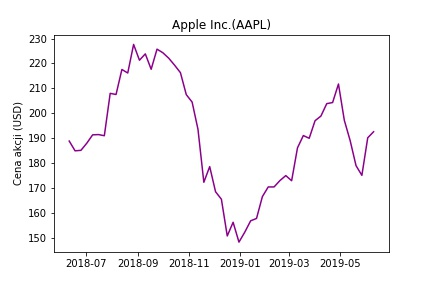
\includegraphics[scale=1]{apple_akcje.jpg}
\caption{Tygodniowe ceny zamknięcia dla akcji Apple Inc. Dane zostały wzięte z giełdy amerykańskiej od 11.06.2018 do 10.06.2019.}
\label{fig:apple_akcje}
\end{figure}
 
Następne symulacje przeporwadzono dla danych z 07.06.2019. Zostały one zaprezentowane w tabeli \ref{tab:dane_apple}.

\begin{table}[h!]
\caption{Dane dla Apple na dzień 07.06.2019}
\centering
\begin{tabular}{|c|c|}
\hline                       
\textbf{Parametr} & \textbf{Wartość} \\
\hline
$S_0$&190.15\\
K&195\\ %przykladowe
$\sigma$&15.50\%\\ %wzięte VIX volatility 
r&2.25\%\\ %amerykańska interest rate
\hline 
\end{tabular}
\label{tab:dane_apple} 
\end{table}

\subsection{Wyniki}

W tabeli \ref{tab:wycena_apple_b} przeprowadzono analizę dla różnych wartości $b$, aby zobaczyć czy estymatory zbiegają do siebie wraz ze wzrostem ilości gałęzi. Pozostałe dane wzięte z tabeli \ref{tab:dane_apple}, a $r_1 = 1$\% i $r_2 = 3$\%, a próg zmiany oprocentowania został ustalony na poziomie $180$.

\begin{table}[h!]
\caption{Porównanie wyestymowanej i 'prawdziwej' ceny opcji amerykańskiej sprzedaży typu omega clock dla różnych ilości gałęzi $b$.}
\centering
\begin{tabular}{cccc}
\hline                       
 & \textbf{Dolny estymator} & \textbf{Górny estymator} & \textbf{Cena}\\
\textbf{b} & \textbf{$\Phi$} & \textbf{$\Theta$} & \textbf{estymowana}\\
\hline
25&12.876&13.554&13.215\\
50&12.683&13.066&12.874\\
75&12.73&13.019&12.875\\
100&12.842&13.077&12.959\\
125&12.744&12.978&12.876\\
\hline 
\end{tabular}
\label{tab:wycena_apple_b} 
\end{table}

Wnioski z tabeli \ref{tab:wycena_apple_b} są podobne jak z tabeli \ref{tab:wycena_am_b}. Również w tym przypadku wartości estymatorów dolnego i górnego są bliższe sobie wraz ze wzrostem $b$, zatem są coraz bliższe jednej cenie. Można zatem wnioskować, że zbiegają do faktycznej sprawiedliwej premii opcji.

Na kolejnych wykresach przedstawiono zależność premii opcji wraz ze zmianą progu zmiany ceny $x$ ze wzoru (\ref{eq:omega}) w przedziale $[130,250]$, a także zależność premii opcji dla zmiennych $r_1$ i $r_2$ (ze wzoru (\ref{eq:omega})) brane odpowiednio w przedziałach $[0,2.25\%$] i $[2.25\%,4.25\%]$.

\begin{figure}[h!]
\centering
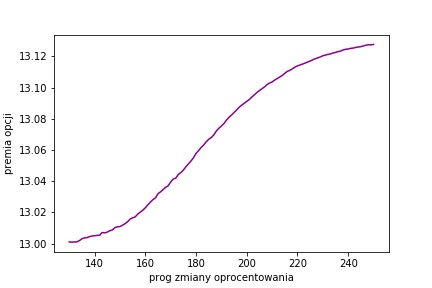
\includegraphics[scale=0.9]{apple_zmienny_prog_2.jpg}
\caption{Wycena amerykańskiej opcji sprzedaży typu omega clock dla zmiennej wartości progu $x$ do zmiany oprocentowania zgodnie ze wzorem \ref{eq:omega}. Wartość progu $x \in [130,250]$.}
\label{fig:apple_prog}
\end{figure}

\begin{figure}[h!]
\centering
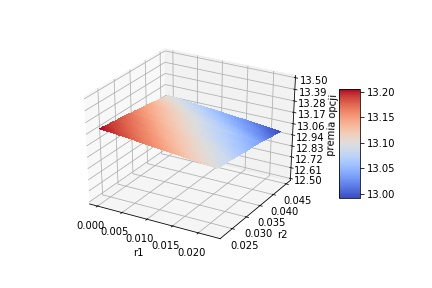
\includegraphics[scale=1.1]{apple_zmienne_r1_i_r2.jpg}
\caption{Wycena amerykańskiej opcji sprzedaży typu omega clock dla zmiennych wartości oprocentownia $r_1$ i $r_2$ ze wzoru \ref{eq:omega}. Wartości tych stóp procentowych $r_1 \in [0,2.25\%]$, $r_2 \in [2.25\%,4.5\%]$.}
\label{fig:apple_zal_r1_r2}
\end{figure}

Na podstawie wykresu \ref{fig:apple_zal_r1_r2} wnioskujemy, że cena maleje wraz ze wzrostem stóp procentowych, co jest zgodne z intuicją.

%{\backmatter \chapter{Podsumowanie}}
%Podsumowanie w pracach matematycznych nie jest obligatoryjne. Warto jednak na zakończenie krótko napisać, co udało nam się zrobić w pracy, a czasem także o tym, czego nie udało się zrobić.

%{\backmatter \chapter{Dodatek}}
%Dodatek w pracach matematycznych również nie jest wymagany. Można w nim przedstawić np. jakiś dłuższy dowód, który z pewnych przyczyn pominęliśmy we właściwej części pracy lub (np. w przypadku prac statystycznych) umieścić dane, które analizowaliśmy.

%%%%%%%%%%%%%%%%%%%%%%%%%%%%%%%%%%%%%%%%%%%%%%%%%%%%%%%%%
% BIBLIOGRAFIA
% W tworzeniu bibliografii najlepiej korzystać z BibTex'a, 
% który jest częścią systemu Tex. W naszym przypadku funkcję 
% przechowalni literatury, do której się odwołujemy, pełni 
% plik bibliografia.bib. Nie musimy ręcznie dodawać nowych 
% pozycji do bibliografii. Możemy wejść np. na stronę 
% https://mathscinet.ams.org/mathscinet/index.html, 
% znaleźć odpowiednią pozycję, wybrać ją, a następnie zmienić 
% 'Select alternative format' na BibTeX, skopiować uzyskany 
% tekst, wkleić do pliku bibliografia.bib i skompilować. 
% Gotowe informacje do pliku bibliografia.bib można znaleźć 
% także na https://arxiv.org - gdy znajdziemy interesującą nas 
% pracę, szukamy 'References & Citations' i klikamy 'NASA ADS', 
% a potem 'Bibtex entry for this abstract' 
% i postępujemy tak jak wcześniej.
%%%%%%%%%%%%%%%%%%%%%%%%%%%%%%%%%%%%%%%%%%%%%%%%%%%%%%%%%
\newpage
% w nawiasie klamrowym wpisujemy nazwę pliku z bibliografią w formacie .bib
\bibliografia{bibliografia} 
\end{document}